\documentclass{article}
\usepackage[utf8]{inputenc}

\usepackage{cmsrb}
\usepackage[T2A]{fontenc} % enable Cyrillic fonts
\usepackage[serbian]{babel}
\usepackage{graphicx}

\title{Минимална сума кластеровања у к кластера\\ \small{Семинарски рад на курсу рачунарска интелигенција \\Математички факултет}}
\author{Михајло Илић}
\date{Септембар 2022}

\begin{document}

\maketitle

\tableofcontents

\newpage
\section{Увод}
\subsection{Кластеровање уопштено}
Појам кластеровања се односи на категоризацију скупа на подскупове такве да елементи у тим подскуповима су сличнији једни другима по неком критеријуму од елемената из других подскупова. Формалније циљ је категоризација елемената u подскупове тако да се максимизује хомогеност елемената истог подскупа и да се такође максимизује хетерогеност елемената из различитих подскупова.\\\\Кластеровање може да се изврши на много начина са неколико начина представљања кластера. Кластеровање као резултат враћа коначан број кластера , док је тај број могуће унапред задати или ослонити се на методу да сама нађе одговаралући број кластера. Сами кластери могу да се представљају са неким репрезентативним елементом нпр. медијаном где би елементи онда припадали том кластеру ако су ближи њему од медијана осталих кластера. Могу да се преклапају међусобно или да буду дисјунктни.\\\\Проблеми у којима се користи метода кластеровања је у ситуацији када је потребно груписати елементе на основу неког критеријума или уочити елементе који се много разликују од било које друге групе елемената.

\subsection{Pregled problema}
Проблем кластеровања у к кластера минималне суме као задатак има проналажење к кластера таквих да сума удаљености елемената унутар тих кластера буде минимална. Потребно је решити следећи оптимизациони проблем:

\begin{displaymath}
\min \sum_{k}^{K}\sum_{j=1}^{n-1}dist(x_{кj},x_{кj+1})
\end{displaymath}
\\К представља скуп кластера, н представља број елемената у к-том кластеру, dist представља метрику за одређивање удаљености два елемента.

\newpage
\section{Opis resenja}
Проблем је решен коришћењем генетског алгоритма за кластеровање. Поред датог алгоритма коришћено је још пар алгоритама ради поређења резултата. Сваки од алгоритама користи помоћну структуру података у виду парцијалне матрице удаљености између елемената. При инизијалицазији алгоритама прво се одреде све удаљености и сместе у ту структуру како би се касније сваки пут кад је потребно наћи удаљеност могло узети одмах из те структуре. Алгоритми генерално раде у месту тј. структуре које користе једанпут само иницијализују у меморији и раде над њима. Ово је урађено како не би било временског губитка због алокације нове меморије. У наредним корацима ће за сваки алгоритам бити објашњено како је имплементиран као и више речи о њему.

\subsection{Kombinatorni algoritam grube sile}
Комбинаторни алгоритам грубе силе је имплементиран као алгоритам апсолутне претраге целог простора могућих решења и враћањем оне инстанце која најбоље испуњава малопре наведену формулу.
Решење се представља у виду низа целих бројева где сваки број означава припадност кластеру елемента на том месту.
\begin{displaymath}
1,1,2,2,3,3,1
\end{displaymath}
Алгоритам ради тако што изгенерише све могуће варијације са понављањем класе к задате дужине и од њих враћа најбољу.
\\\\Предност овох приступа је што ће сигурно наћи најбоље решење и лак је за имплементацију, међутим временски је неефикасан до те мере да већ за троцифрен број елемената алгоритам није употребљив у разумном окружењу.
Такође једна од могућности и погодност овог алгоритма је лака паралелизација.
Због унапред познатог броја варијација и могућности одређивања специфичне варијације алгоритам може да се убрза тако што ће се поделити на $n$ послова где ће сваки обрађивати један део од скупа варијација.
Овим приступом једини дељени ресурс о ком би се водило рачуна је оптимална варијација.

\subsection{Pohlepni algoritam}
Похлепни алгоритам представља унапређење технике грубе силе где уместо претраге целог скупа решења алгоритам се наводи и тиме узима у обзир само један део већег скупа решења.
Користи исту репрезентацију за припадност елемената кластерима као и алгоритам грубе силе, међутим користи малу оптимизацију у виду чувања локалних сума унутар сваког кластера.
За кластеровање са к кластера алгоритам чува низ реалних бројева дужине к где памти удаљености између елеманата у датом кластеру.
Разлог за таквом имплементацијом је рад алгоритма.
\\\\Креће се тако што се иницијални скуп елемената додели сваком од к кластера.
Затим све док се не испуни услов за завршетак рада алгоритма покушава пронаћи следеће најбоље решење тако што ће поправити тренутно.
Поправка се ради тако што за сваки елемент покуша да га премести у други кластер и ако се сума смањи узима њега за тренутно решење.
Рачунање суме не ради сваки пут него само ажурира кластере који се мењају.
\\\\Предност овог алгоритма је та што за разлику од алгоритма грубе силе понаша се боље за већи број елемената који требају да се кластерују.Његова мана је та што не гарантује оптимално решење. Могуће је да уместо глобалног оптимума алгоритам врати локални.
\subsection{Genetski algoritam}
Алгоритам којим смо одабрали да решимо проблем је генетски алгоритам прилагођен за проблеме кластеровања.
Алгоритам опонаша процес еволуције и природне селекције тако што симулира преживљавање и размножавање најпогоднијих јединки из популације кроз неколико генерација са циљем да на крају испливају најпогодније јединке.
Категорисање колико је јединка погодна се врши представљањем решења као генотипа јединке и квантификацијом тог генотипа.
Након тога упоређивање две јединке је могуће и оно што је остало је одабир и укрштање погодних.
Уопштено алгоритам је имплементиран тако да насумично генерише насумичну иницијалну популацију над којом се примењује процес природне селекције кроз задати број генерација.
Алгоритам имплементира елитизам ради опстајања једног дела најбољих јединки у следећој генерацији , како се не би потенцијално изгубило добро решење.
Кроз операторе укрштања и мутације теоријски могуће је добити неповољне генотипе у смислу добијања генотипа где неки кластер нема додељен елемент.
Алгоритам о томе не води рачуна ради због једноставности.
Могуће је додати операције које ће се бринути да су сва решења из повољног скупа решења или поправком или одбацивањем таквих решења или чак додељивањем мањег фитнеса у нади да ће таква решења природно изумрти.
У наредним деловима биће објашњени детаљи око имплементације овог алгоритма.

 \subsubsection{Reprezentacija jedinke}
 Свака јединка је имплементирана тако што као и у претходним алгоритмима њен генотип је представљен као низ целих бројева који представљају додељене кластере инстанци на том месту.
 Погодност овакве репрезентације је та што се лако имплементира и лако се имплементирају оператори укрштања и мутације над њом.
 Велика мана је та што оваква приступ кодирања решења заузима много меморије јер за сваку јединку чувамо потенцијално велик низ целих бројева.
 Могућа оптимизација може да укључи да уместо низа бројева којем кластеру припадају елементи чувамо само центре кластера.
 Тако би знатно смањили меморијски трошак алгоритма јер генерално је тражени број кластера к мањи од броја елемената.
 Мана таквог приступа је што отежава остале операторе и теже их је имплементирати за овај специфичан проблем.
 
 \subsubsection{Фитнес функција}
 За фитнес функцију је одабрана реципрочна вредност почетне функције.
 Разлог за то је што је циљ проблема да се минимизује почетна функција, а генетски алгоритам максимизује фитнес функцију.Тако да што је укупна сума мања фитнес неке јединке је бољи што и желимо.
 
 \begin{displaymath}
fitness(X) = \frac{1}{\sum_{k}^{K}\sum_{j=1}^{n-1}dist(x_{кj},x_{кj+1})}
\end{displaymath}
 
 \subsubsection{Ukrstanje}
 За укрштање две јединке и креирање нових јединки је изабрано једнопозиционо укрштање где би се одабрала произвољна тачка у генотипу родитеља и унакрсним спајањем тако подељених генотипа родитеља креирала деца.
 Погодност оваквог оператора укрштања је та што је лак за имплементацију и даје повољне резултате.
 Једна од мана је та што теоријски може да креира неповољне генотипе у контектсту проблема.
 Наиме може да креира репрезентацију где неком кластеру није додељена ниједна јединка.
 Већа је вероватноћа да се овако нешто деси у мањим генотипима него у дужим.
 
 \subsubsection{Mutacija}
 За оператор мутације је насумично одабран један елемент из генотипа и додељен другом кластеру.
 
\section{Eksperimentalni rezultati}
Као експеримент узет је стандардни скуп са латицама и скуп ruspini за кластер анализу.
Алгоритам грубе силе већ није у могућности да произведе резултат у нормалном временском интервалу док похлепни алгоритам и генетски успевају да дају исте резултате. 

\newpage

\begin{table}[h!]
  \begin{center}
    \caption{Табела за скуп са латицама}
    \label{tab:table1}
    \begin{tabular}{l|c|r}
      \textbf{алгоритам} & \textbf{минимална сума} & \textbf{време извршавања}\\
      \hline
      груба сила & / & /\\
      похлепни & 3406 & 3.89\\
      генетски & 3406 & 93.84\\
    \end{tabular}
  \end{center}
\end{table}

\begin{table}[h!]
  \begin{center}
    \caption{Табела за скуп руспини}
    \label{tab:table1}
    \begin{tabular}{l|c|r}
      \textbf{алгоритам} & \textbf{минимална сума} & \textbf{време извршавања}\\
      \hline
      груба сила & / & /\\
      похлепни & 10956 & 1.14\\
      генетски & 10956 & 20.59\\
    \end{tabular}
  \end{center}
\end{table}

\begin{table}[h!]
  \begin{center}
    \caption{Табела за насумичан скуп}
    \label{tab:table1}
    \begin{tabular}{l|c|r}
      \textbf{алгоритам} & \textbf{минимална сума} & \textbf{време извршавања}\\
      \hline
      груба сила & / & /\\
      похлепни & 2851536 & 562\\
      генетски & 2850149 & 290\\
    \end{tabular}
  \end{center}
\end{table}

\begin{figure}
    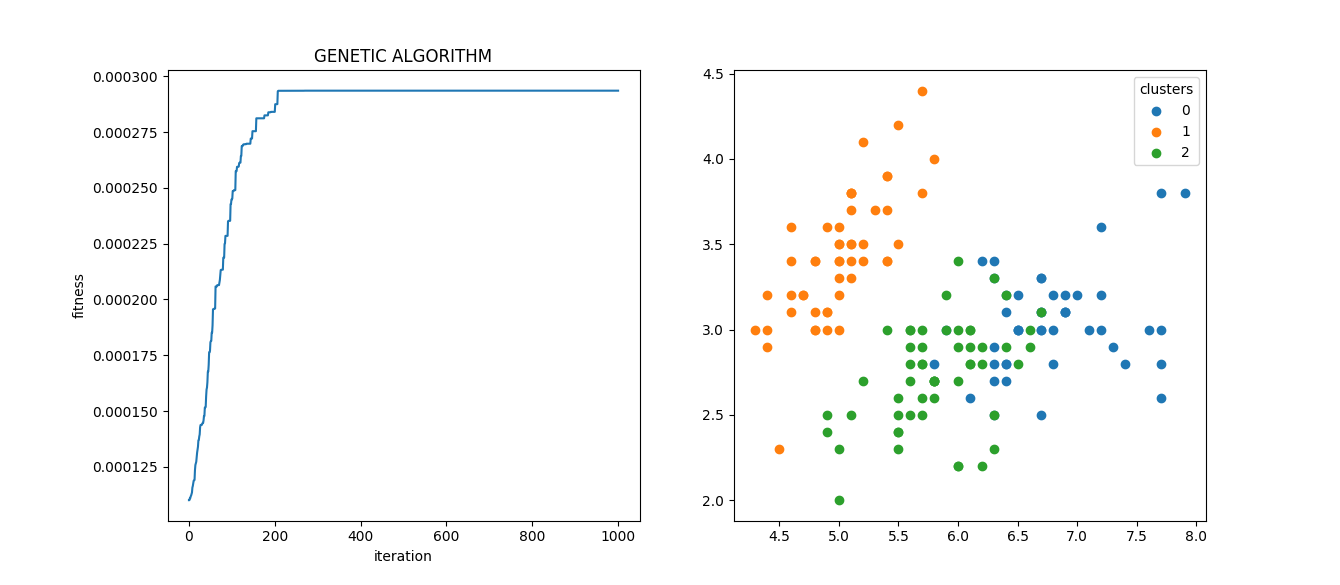
\includegraphics[width=\textwidth]{genetic_iris.png}\hfill
    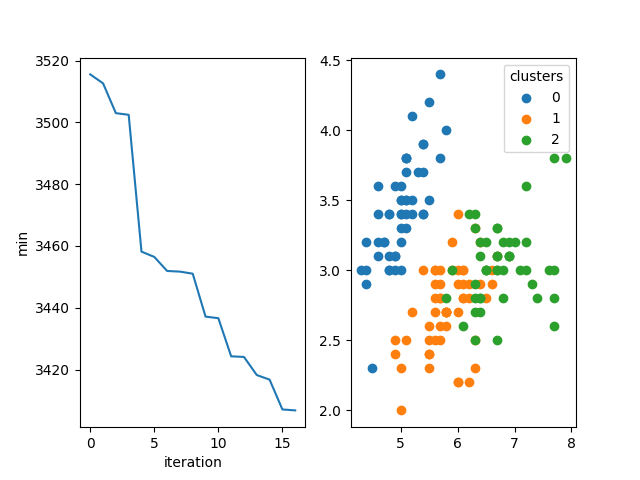
\includegraphics[width=\textwidth]{greedy_iris.png}\hfill
    \caption{Скуп са латицама}\label{fig:foobar}
\end{figure}

\begin{figure}
    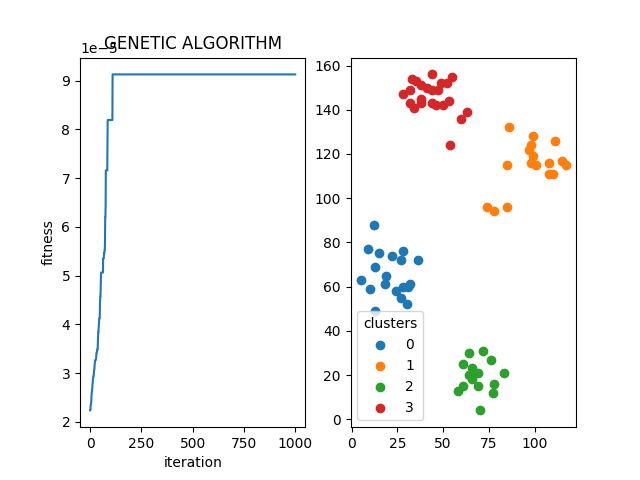
\includegraphics[width=\textwidth]{genetic_ruspini.png}
    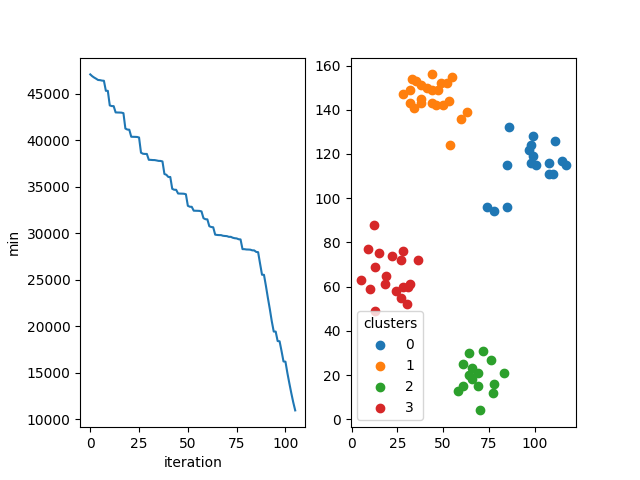
\includegraphics[width=\textwidth]{greedy_ruspini.png}
    \caption{Руспини скуп}\label{fig:foobar}
\end{figure}

\begin{figure}
    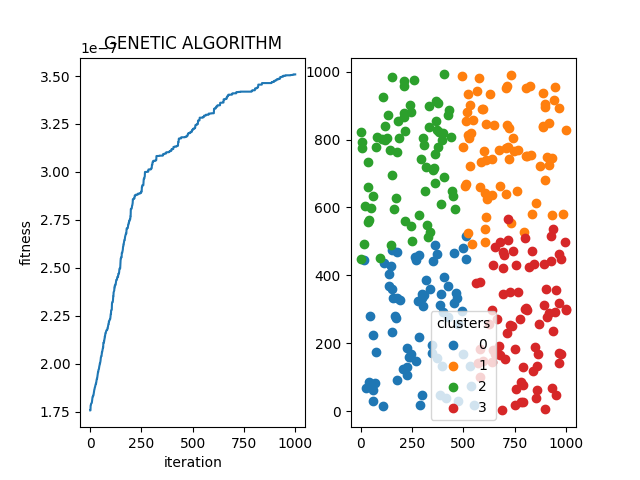
\includegraphics[width=\textwidth]{genetic_random.png}
    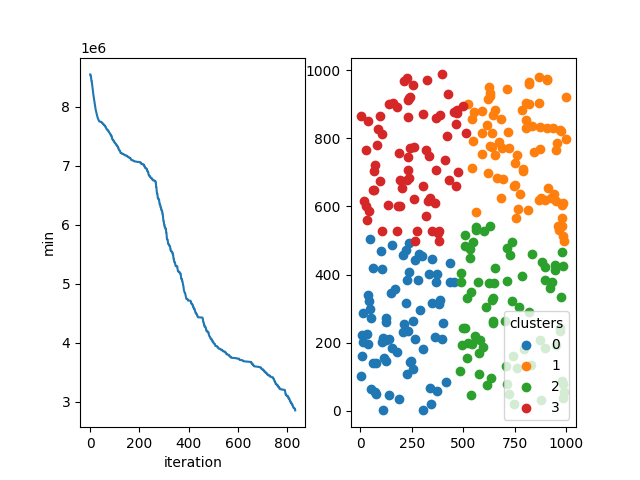
\includegraphics[width=\textwidth]{greedy_random.png}
    \caption{Насумичан скуп}\label{fig:foobar}
\end{figure}

\newpage
\section{Закључак}
Похлепни алгоритам се понаша најбоље у односу на друге алгоритме за мале и једноставне улазе.
Док генетски алгоритам понаша боље за велике и комплексније скупове података.
Алгоритам грубе силе већ за скупове са стотину инстанци не усепва у разумном року да пронађе минималну суму.
Такође предност која се очекује од генетског алгоритма у односу похлепни је мања вероватноћа упадања у локални екстремум
због оператора укрштања и мутације који му пружају могућност истраживања више решења.
Генетски алгоритам такође може да се унапреди тако што ће се извршити симулирано каљење или на крају рада или на неколико
најбољих јединки на крају сваке генерације.


\addcontentsline{toc}{section}{Literatura}
\appendix

\newpage

\iffalse
\bibliography{seminarski} 
\bibliographystyle{plain}
\fi

\begin{thebibliography}{Literatura}
Није била пронађена бесплатна литература на ову тему
\end{thebibliography}


\end{document}
